\chapter{面向异构后端的容器内存压力感知卸载架构总体设计}

本章首先说明系统的设计,然后介绍介绍整体系统的架构、内核态和用户态的各个模块和组件,各个模块之间的交互,以及整个框架的执行流程。

\begin{figure}[h]
    \centering
    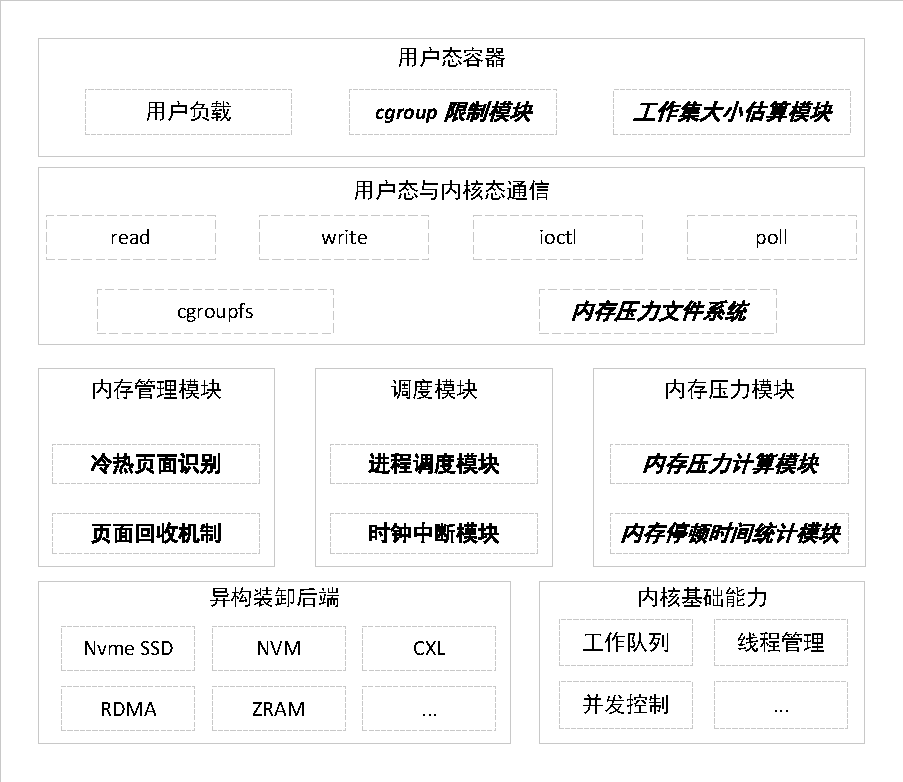
\includegraphics[width=0.8\textwidth]{架构层次图.pdf}
    \caption{架构层次图}
    \label{fig:system_architecture_hierarchy}
\end{figure}

\section{需要分析与设计目标}

本系统旨在为异构后端提供一个基于内存压力感知的透明卸载的框架,只需要将异构装卸后端接入到基于Linux的换入后端中,就可以实现内存压力感知的透明卸载。有很高的拓展性,无需要每种不同的异构后端实现工作集的计算

该系统采用了一种新颖的内核态-用户态协同方法,以实现对内存压力的精确感知和对容器工作集的动态优化。本研究将内存压力定义为由于内存资源不足而导致的应用程序性能下降,具体表现为同步内存回收操作所占用的时间片比例。基于此,我们首先在内核层构建了一个细粒度的内存压力模型,该模型能够实时、准确地反映系统的内存受限程度;基于该模型,我们在用户态设计了一种自适应的工作集估计算法,该算法能够根据内存压力动态调整容器的内存资源分配。

具体而言,本系统的设计目标涵盖以下功能性需求:

\begin{itemize}
    \item \textbf{内存压力感知:} 内核态模块需要能够精确、实时地监测系统的内存压力,并将压力信息传递给用户态模块。
    \item \textbf{工作集估计与调整:} 用户态模块需要根据内核态提供的内存压力信息,动态估算容器的工作集大小,并据此调整容器的内存资源限制。
    \item \textbf{冷热页优化:} 框架需要优化冷热页面的识别机制,能够根据不同的工作负载特性,动态调整文件页和匿名页的回收比例。
    \item \textbf{透明卸载:} 卸载过程对用户态应用程序透明,无需修改应用程序代码。新的卸载后端设备应能通过标准接口(如扩展 swap 文件系统)接入系统。
\end{itemize}

在非功能性需求方面,主要有以下几点:

\begin{itemize}
    \item \textbf{内存节省:} 框架自身的内存开销应尽可能小,以避免对系统造成额外的内存负担。
    \item \textbf{低计算开销:} 内存压力计算和工作集估计算法的计算复杂度应尽可能低,以减少对 CPU 资源的占用。
\end{itemize}


通过实现上述设计目标,本系统将为容器化环境提供一种高效、灵活、透明的内存压力管理方案,显著提升容器在内存受限场景下的性能和资源利用率。

\section{系统架构}

本论文提出的面向异构后端的容器内存压力感知卸载框架的系统架构如图 \ref{fig:system_architecture_hierarchy} 所示。该框架采用内核态-用户态协同设计模式,旨在实现对容器内存压力的精确感知与动态卸载。图中加粗斜线表示新增模块,加粗部分表示修改模块。

框架底层由异构卸载后端和内核基础能力构成。异构卸载后端支持多种存储设备,包括NVMe SSD、NVM、CXL、RDMA和ZRAM等,可通过扩展swap文件系统实现不同后端的接入。内核基础能力为框架运行提供必要支持,涵盖工作队列、线程管理及并发控制等核心功能。

框架的核心组件为内核态模块,由三个主要子模块构成:内存管理模块、进程管理模块和内存压力模块。内存管理模块包含冷热页面识别、页面分配与回收机制,其中冷热页面识别与页面分配模块已进行优化改进;进程管理模块包含进程管理与调度功能,已实现相应改进;内存压力模块由内存压力计算与内存停顿时间统计组成,均为新增模块。内核态模块深度集成于Linux内核的内存管理子系统,通过扩展页面分配、页面回收及进程调度机制,实现对内存压力的细粒度监测与控制。具体而言,内存压力模块实时计算系统内存压力指标,并通过用户态与内核态通信模块(mpfs)向用户态提供相关信息。进程管理模块则依据内存压力状况,动态调整进程调度策略,以优化系统整体性能。

用户态容器包含三个核心模块:用户负载、cgroup限制模块及工作集大小估算模块。用户负载代表容器内运行的实际应用程序;cgroup限制模块基于Linux内核的cgroup机制,对容器内存资源使用进行约束;工作集大小估算模块根据内核态提供的内存压力信息,动态估算容器工作集大小,并据此调整cgroup内存限制,实现容器内存资源的优化分配。

用户态与内核态之间通过多种通信机制实现交互。除利用cgroupsfs进行cgroup配置外,还可使用标准系统调用接口,如`read`、`write`、`ioctl`和`poll`。此外,通过自定义的`mpfs`(memory pressure file system)接口,可实现更高效、灵活的通信。用户态应用程序可借助这些通信机制获取内核态内存压力信息,并对容器内存资源配置进行动态调整。

本节后续内容将详细阐述系统各模块的功能与职责。


\subsection{内存压力模块}

内存压力模块作为本框架的核心组件,承担着将内核检测到的内存短缺状况进行量化表征的关键任务,为用户态的资源调度与优化决策提供数据支撑。该模块采用动态监测与分析机制,构建了多维度的内存压力评估模型,而非提供单一瞬时压力值。

内存压力模块的核心组件为内存停顿时间统计单元。该单元通过在内核同步内存回收路径上实施精细化插桩,捕获因内存分配请求无法立即满足而触发的同步回收事件。对于每个同步回收事件,系统精确记录其起始时间、终止时间以及期间发生的并发事件(如进程调度、中断处理等),进而计算该回收操作占用的CPU时间片。然后和调度系统交互,得到分配的时间片,最后得到比例。这种时间片比例直接反映了内存子系统处理内存短缺对程序执行造成的延迟影响。值得注意的是,统计范围仅限于同步回收导致的停顿,因为异步回收通常不会直接阻塞应用程序执行。

内存压力计算单元基于内存停顿时间统计单元提供的原始数据,采用加权平均、滑动窗口、指数衰减等统计方法进行多维度分析。该单元不仅考虑最近一次停顿时间,还综合历史数据,生成能够平滑反映内存压力变化的量化指标。该指标设计旨在平衡响应速度与稳定性,既能够及时捕捉内存压力突变,又可避免因短期波动导致的误判,从而为用户态提供可靠的决策依据。

\subsection{通信模块}

通信模块负责实现内核态与用户态之间的高效数据交互,确保内存压力指标能够实时、准确地传递至用户态的容器管理组件。本模块基于proc虚拟文件系统实现,通过创建特定入口(如/proc/mem_pressure)以标准文件I/O操作方式暴露内存压力信息。该入口采用结构化数据格式(如百分比)呈现内存压力指标,用户态程序可通过read系统调用直接获取相关信息。

为支持用户态程序对内存压力变化的实时响应,通信模块实现了poll系统调用接口。该接口采用事件驱动模型,允许用户态程序注册对特定文件描述符(即内存压力信息入口)的事件监听。当内存压力指标超过预设阈值时,内核通过poll机制主动通知用户态程序,有效避免了频繁轮询带来的性能开销。这种事件驱动设计显著提升了用户态程序响应内存压力变化的及时性与效率。

\subsection{用户态容器}

用户态容器作为应用程序运行的隔离环境,是本框架实现内存压力感知与动态资源调整的执行单元。容器架构包含以下核心组件:

用户负载组件代表容器内运行的实际应用程序或服务。这些应用程序对底层的内存压力感知与资源调整机制保持透明,无需任何修改即可受益于框架提供的性能优化。

工作集大小估算模块是容器的关键组件,负责基于通信模块提供的内存压力信息,动态评估容器的当前工作集大小(即应用程序正常运行所需的最小内存量)。该模块采用启发式算法,综合考虑容器的历史内存使用模式、当前内存压力水平、应用程序类型与行为特征等因素,生成容器的理想内存需求评估结果。

cgroup限制模块利用Linux内核的cgroup机制,对容器的内存资源使用实施动态约束。该模块通过与cgroupsfs文件系统交互,实时调整容器的内存硬限制(memory.limit_in_bytes)和软限制(memory.soft_limit_in_bytes)等参数。工作集大小估算模块的输出作为cgroup限制模块的核心输入,指导其设置合理的内存限制,在保障容器性能的同时优化系统资源利用率。

\subsection{内存管理模块}

内存管理模块作为Linux内核的核心组件,负责系统物理内存的分配、回收与维护。本框架重点优化了冷热页面识别机制,提升了内存管理的效率与准确性。
冷热页面识别机制是内存回收和页面置换策略的基础。传统 Linux 内核的内存回收机制在设计时,为了尽可能减少对系统性能的影响,倾向于优先回收文件页(file-backed pages)。这是因为文件页通常可以从磁盘重新读取,而匿名页如果被换出到交换分区(swap),则在重新换入时可能需要更长的延迟。

此外,为支持内存压力模块的统计需求,本框架在内存分配与回收的关键路径上实施了插桩,用于收集分配延迟、回收延迟等详细内存操作信息,为系统性能分析与优化提供了数据支撑。


\section{运行流程}

本节介绍系统运行流程,从框架初始化以及用户态和内核态的交互流程来介绍内存压力模块以及用户态容器组成的完整系统的典型流程,以进一步说明各个模块的之间的关系。

\begin{figure}[h]
    \centering
    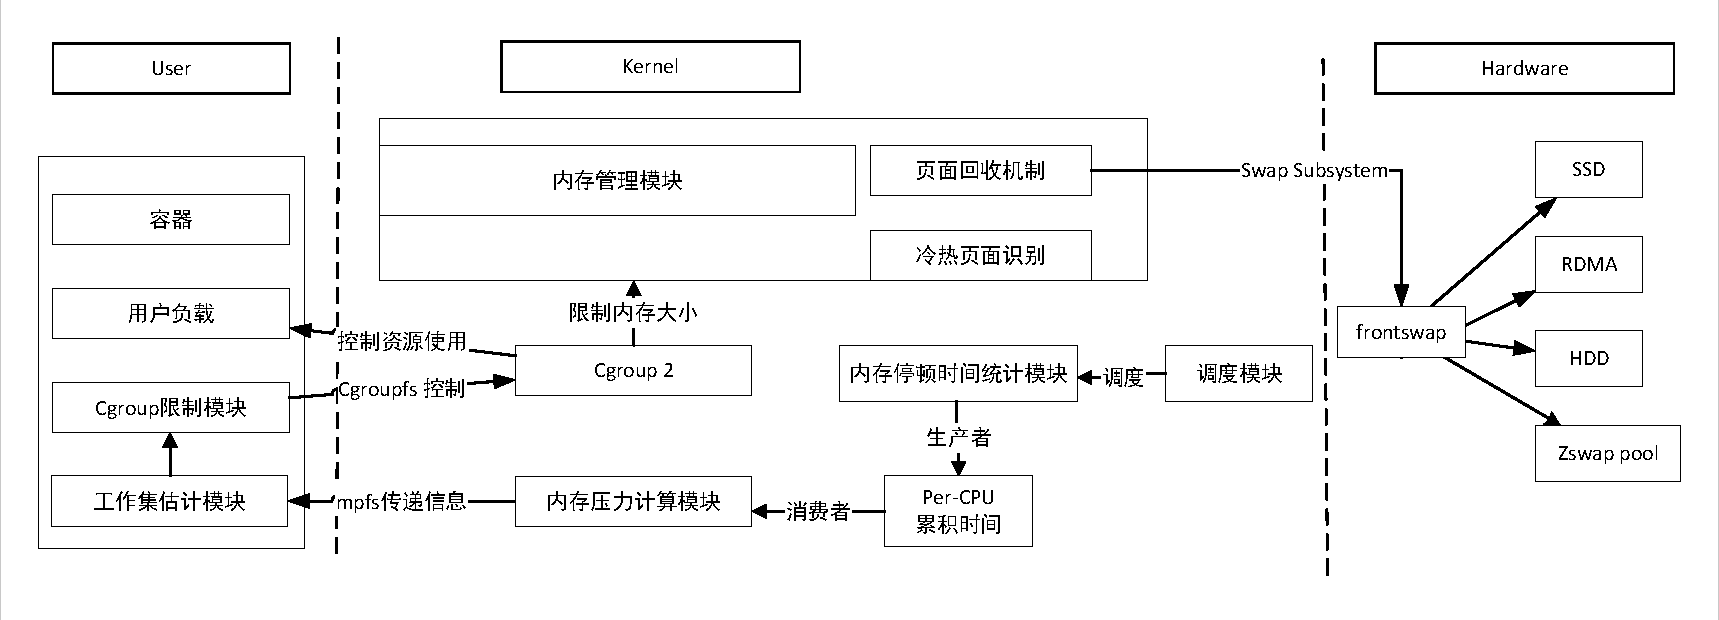
\includegraphics[width=0.8\textwidth]{架构图.pdf}
    \caption{系统整体架构}
    \label{fig:system_architecture}
\end{figure}

\subsection{框架初始化}

\begin{figure}[h]
    \centering
    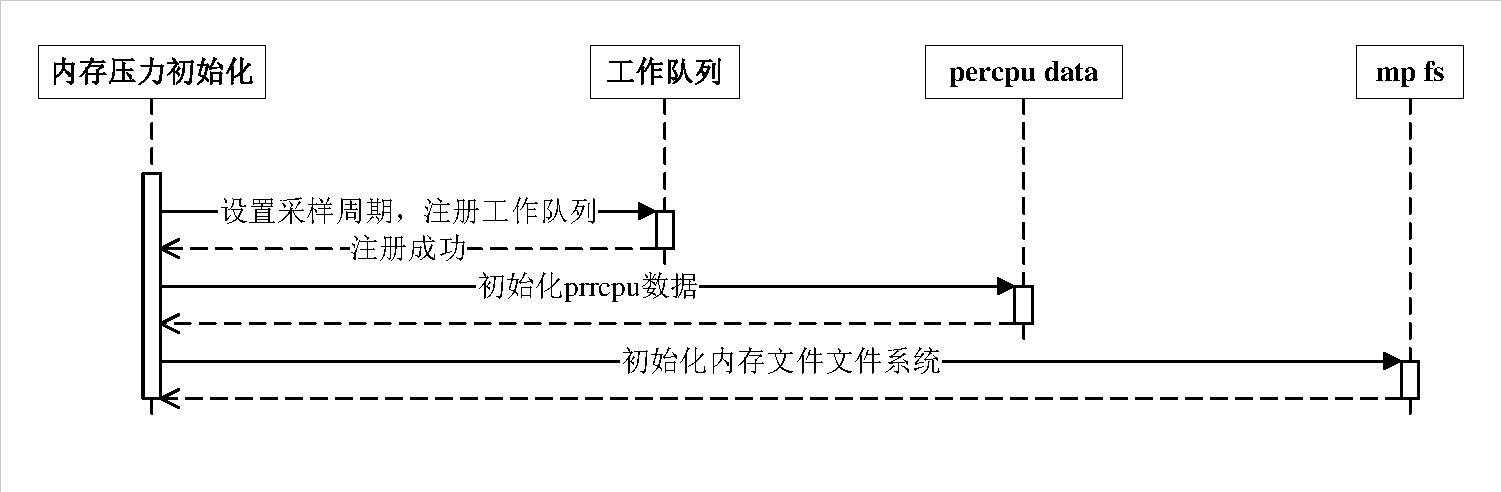
\includegraphics[width=0.8\textwidth]{mp初始化.pdf}
    \caption{框架初始化}
    \label{fig:framework_initialization}
\end{figure}

框架初始化流程是系统构建的基石,为后续的内存压力监控与管理奠定稳固基础。如图 \ref{fig:framework_initialization} 所示,初始化流程主要包含以下几个紧密相连的关键阶段:

首先,系统启动后,会立即进入采样周期与工作队列的配置环节。这一阶段的核心在于为内存压力的周期性监控设定合适的参数。采样周期的选择至关重要,它直接决定了系统对内存压力波动响应的灵敏程度。若采样周期设置过长,则可能错过内存压力的瞬时尖峰,导致无法及时采取应对措施;反之,过短的采样周期会频繁触发数据收集和计算,给系统带来不必要的性能开销。因此,一个合理的采样周期需要在捕捉内存压力变化和降低系统负担之间取得精妙的平衡,这通常需要根据系统的实际负载特性和性能需求进行动态调整。同时,为了避免在中断上下文中执行可能耗时的操作(这会严重影响系统的实时性和稳定性),内核广泛采用工作队列机制来实现任务的异步执行。本框架充分利用了工作队列的优势,将内存压力的统计、计算、以及向用户态报告等一系列相关任务都交由工作队列异步处理。在具体实现上,系统通过内核提供的配置接口(如 sysctl)或模块参数来设置采样周期,并创建一个专用的内核工作队列,将与内存压力处理相关的函数注册到该队列。在每个采样周期结束时,内核会触发工作队列中注册的处理函数,从而启动新一轮的内存压力信息收集与计算流程。

其次,虽然在初始化阶段会为每个 CPU 核心分配并初始化 per-CPU 变量,但这些变量在此时并不会立即投入使用。per-CPU 变量主要用于存储每个 CPU 核心上的内存压力相关统计信息,包括停顿时间、分配延迟等关键指标,以及一些用于辅助计算和同步的元数据。这些 per-CPU 变量的设计充分考虑了数据局部性和访问效率,旨在减少跨 CPU 访问和锁竞争,从而提升系统整体性能。然而,这些变量的初始值仅仅是占位符,其真正发挥作用是在后续的内存回收阶段。在发生内存回收事件时,相关的内核路径会更新对应 CPU 核心上的 per-CPU 变量,记录下详细的停顿时间和其它相关信息。随后,工作队列中的处理函数会定期读取这些 per-CPU 变量,并进行综合分析和计算,最终得出反映系统整体内存压力的指标。这种设计将数据的收集和计算解耦,避免了在内存回收的关键路径上引入过多的性能开销。

最后,系统会着手初始化并挂载 mpfs(Memory Pressure File System)文件系统。mpfs 作为本框架实现内核态与用户态高效通信的核心组件,其本质是一个驻留在内存中的虚拟文件系统,不涉及任何磁盘 I/O 操作,从而确保了极低的访问延迟。通过调用内核提供的 mount 系统调用,mpfs 文件系统会被挂载到预先指定的目录(通常为 /sys/fs/mpfs)。在挂载过程中,内核会创建一系列内部数据结构来表示 mpfs 文件系统,并将其与 VFS(Virtual File System)层紧密集成。与此同时,mpfs 文件系统自身的一些元数据信息,如 inode 信息、文件操作函数指针等,也会在这一阶段被初始化。这些元数据信息定义了 mpfs 文件系统的行为和特性,使其能够正确响应用户态的文件操作请求。通过 mpfs,内核可以将内存压力信息以标准文件的形式暴露给用户态,而用户态程序可以通过常规的文件操作(如 read、poll 等)便捷地获取这些信息,从而实现对系统内存压力的实时监控和响应。


\subsection{用户态和内核态的交互流程}

用户态和内核态共同作用将内存卸载的过程

